% Prepared by Calvin Kent
%
% Assignment Template v19.02
%
%%% 20xx0x/MATHxxx/Crowdmark/Ax
%
\documentclass[12pt]{article} %
\usepackage{CKpreamble}
\usepackage{CKassignment}
\usepackage{tkz-euclide}
\usepackage{physunits}
\usepackage{physics}
\usepackage{lmodern}
\usepackage{microtype}
\usepackage{upgreek}
\usepackage[misc]{ifsym}


%%Title
\title{Functions Test 1 - SOLUTIONS}
\date{December 14, 2021}

%%% Maths and science packages

\usepackage{amsmath,amsthm,amssymb}
\usepackage{pgfplots}
	\usetikzlibrary{
		calc,
		patterns,
		positioning
	}
	\pgfplotsset{
		compat=1.16,
		samples=200,
		clip=false,
		my axis style/.style={
			axis x line=middle,
			axis y line=middle,
			legend pos=outer north east,
			axis line style={
				->,
			},
			legend style={
				font=\footnotesize
			},
			label style={
				font=\footnotesize
			},
			tick label style={
				font=\footnotesize
			},
			xlabel style={
				at={
					(ticklabel* cs:1)
				},
				anchor=west,
				font=\footnotesize,
			},
			ylabel style={
				at={
					(ticklabel* cs:1)
				},
				anchor=west,
				font=\footnotesize,
			},
			xlabel= $x$,
			ylabel=$\vec d (\m \tx{[East]})$
		},
	}
	\tikzset{
		>=stealth
	}

%%% Tables and figures packages

\usepackage{float}
\usepackage{caption}
	\captionsetup{
		format=plain,
		labelfont=bf,
		font=small,
		justification=centering
	}


\newcounter{step}[section]
\newenvironment{step}[1][]
{\refstepcounter{step} \textbf{\\Step #1.}}
	
%%% Numbers and sets

\newcommand{\E}{\mathrm{e}}

\newcommand{\tx}[1]{\text{#1}}

\begin{document}
    \pagenumbering{arabic}
    % Start of class settings ...
    \renewcommand*{\coursecode}{MCR3U Quiz} % Quiz Title
    \renewcommand*{\assgnnumber}{1} % Quiz number
    \renewcommand*{\submdate}{November, 2021} % renew the date
    \renewcommand*{\studentfname}{\textbf{Name:}} % Student first name
    \renewcommand*{\studentlname}{} % Student last name
    %\renewcommand*{\studentnum}{SNumber} % Student number

    \renewcommand\qedsymbol{$\blacksquare$}
    \setfigpath
    % End of class settings 
    \newgeometry{left=18mm, right=18mm, top=22mm, bottom=22mm} % page is set to default values
    \fancyhfoffset[L,O]{0pt} % header orientation fixed
    % End of class settings
    %%% Note to user:
    % CTRL + F <CHANGE ME:> (without the angular brackets) in CKpreamble to specify graphics paths accordingly.
    % The command \circled[]{} accepts one optional and one mandatory argument.
    % Optional argument is for the size of the circle and mandatory argument is for its contents.
    % \circled{A} produces circled A, with size drawn for letter A. \circled[TT]{A} produces circled A with size drawn for TT.
    % https://github.com/CalvinKent/My-LaTeX
    %%%
    % Crowdmark assignment start


    %%%%%%%%%%%%%%%%%%%%%%%%%%%%%%%%%%%%%%%%%%%%%%%%%%%%%%%%%%%%%%%%%%%%%%%%%%%%%%%%%%%%%%%%%%%%%%%%%%%%%%%%
    %%%%%%%%%%%%%%%%%                  PROBLEM IDEAS                  %%%%%%%%%%%%%%%%%%%%%%%%%%%%%%%%%%%%%%
    %%%%%                   ----------------------------------------                                %%%%%%%%

    % --> Do a hard tangent line problem

	\maketitle
	\section{Preamble}
	This is a test covering what we have learnt so far in lecture. Student's \emph{must show all work} to receive full marks.
	\section{Allowed Aids}
	The following aids are allowed on the Test
	\begin{itemize}
		\item Pencil, Pen, Eraser, Highlighter, Ruler, Protractor, Spare sheets of \textbf{blank} paper.
		\item Reference sheet \textbf{(Double sided paper preprepared by student)}
	\end{itemize}
	\section{Restrictions:}
  \begin{itemize}
		\item \textbf{NO} calculator's.
  \end{itemize}
  \section{Remarks:}
  \begin{itemize}
    \item $\mathbb N = \{1,2,3,4,5,\dots\} $.
    \item $\operatorname{rem}(x,y)$ is the remainder when you divide $x$ by $y$.
  \end{itemize}
	\section{Name and Date:}
	Print your name and todays date below;\\

	\begin{center}
	\noindent\begin{tabular}{ll}
		\makebox[3in]{\hrulefill} & \makebox[3in]{\hrulefill}\\
		Name & Date\\[8ex]% adds space between the two sets of signatures
	\end{tabular}
	\end{center}
	\newpage


\begin{qstn} % qnumber, qname, qpoints
  (10 marks) Answer the following True/False questions,
  \begin{enumerate}
    \item Let $\mathcal{R} = \{4,5,6,7,8\} $ and $\mathcal{H} = \emptyset $, then $\mathcal{R} + \mathcal{H} = \emptyset $.\\
      \textbf{\emph{Answer}}: \,\,\, \textbf{False}, \,\, $\mathcal{R} + \mathcal{H} =   \{4,5,6,7,8\}$.\\

    \item Let $S = \{3,4,5\} $, then $S + S = S$.\\
      \textbf{\emph{Answer}}: \,\,\, \textbf{True}. \,\,\\

    \item $(\sqrt{4} + \pi) \in \Z$.\\
      \textbf{\emph{Answer}}: \,\,\, \textbf{False}, \,\, $(4 + \pi) \in \R$.\\

    \item The vertex of 
      \[
        f(x) = 3\left( x + \pi \right)^2 - \sqrt{16}  
      \] is $(-\pi,-8)$.\\ 
      \textbf{\emph{Answer}}: \,\,\, \textbf{False}, \,\, The vertex is $(-\pi, -4)$.\\

    \item The centre of the circle,
      \[
            (x-1)^2 + (y -2)^2 = 4
      \] is $(-1,-2)$.\\
      \textbf{\emph{Answer}}: \,\,\, \textbf{False}, \,\, The centre of the circle is $(1,2)$.\\

    \item The vertex of,
      \[
            f(x) = -\left( x - 3 \right)^2 - 4
      .\] represents a maximum.\\
      \textbf{\emph{Answer}}: \,\,\, \textbf{True}. \,\,\\

    \item The Domain and Range of,
      \[
              f(x) = -\frac{4}{2x + 1} + 8
    .\] is $\mathcal{D} = \{x \in \R \mid x \neq \frac{1}{2}\} $, $\mathcal{R} = \{y \in \R \mid y \neq 8\} $.\\
      \textbf{\emph{Answer}}: \,\,\, \textbf{False}, \,\,  $\mathcal{D} = \{x \in \R \mid x \neq -\frac{1}{2}\} $, $\mathcal{R} = \{y \in \R \mid y \neq 8\} $.\\

    \item If $\mathcal{V} = \{v \in \mathbb N \mid v^2 = -1\}$, then $\mathcal{V}$ is the empty set.\\
      \textbf{\emph{Answer}}: \,\,\, \textbf{True}. \,\,\\

    \item The x-intercepts of $f(x) = x^2 -5x + 6$ are $x_1 = -2$ and $x_2 = -3$.\\
      \textbf{\emph{Answer}}: \,\,\, \textbf{False}, \,\, The x-intercepts are $x_1 = 2$ and $x_2 = 3$.\\

    \item The vertex of $f(x) = x^2 + 6x + 5$ is $(-3,-4)$. \\
      \textbf{\emph{Answer}}: \,\,\, \textbf{True}. \,\,\\

  \end{enumerate}
\end{qstn}

\newpage

\begin{qstn}
  (4 marks) Write down the elements of the following sets.\\
  (\textbf{Recall:} $\mathbb N = \{1,2,3,4,\dots\} $)
  \begin{enumerate}[label=(\alph*)]
    \item $\mathcal{T} = \{a \in \Z \mid 3 < a < 7\} $.
      \begin{solution}
        $\mathcal{T} = \{4,5,6\} $.
      \end{solution}

      \vspace*{3cm}



    \item $\mathcal{X} = \{x \in \mathbb N \mid x \neq 1 \} $.
      \begin{solution}
        $\mathcal{X} = \{2,3,4,5,6,\dots\} $.
      \end{solution}

      \vspace*{3cm}

    \item $\mathcal{Z} = \{y \in \mathbb Z \mid -3 \leq y \leq 0\} +  \{i \in \mathbb Z \mid -2 \leq i \leq 1\}$ \\
      \textbf{Hint:} Add the two sets first.
      \begin{solution}
        \begin{align*}
          \mathcal{Z} &= \{-3,-2,-1,0\} + \{-2,-1,0,1\}\\
                      &= \{-3,-2,-1,0,-2,-1,0,1\} \tag{Merging}\\
                      &= \{-3,-2,-1,0,1\} \tag{Removing duplicates}
        .\end{align*}
      \end{solution}

      \vspace*{1cm}

    \item $\mathcal{B} = \{x \in \mathbb N \mid \operatorname{rem}(x,2) = 0\} $.
      \begin{solution}
        If you look carefully, all the numbers that satisfy the condition that $\operatorname{rem}(x,2) = 0$ are all of the even
        numbers! Hence,
        \[
            \mathcal{B} = \{2,4,6,8,10,\dots\} 
        .\] 
      \end{solution}

  \end{enumerate}
\end{qstn}

\newpage

\begin{qstn}
  (8 marks) Determine the Domain and Range of the following functions,
  \begin{enumerate}[label=(\alph*)]
    \item $\mathcal{Y}(x) = -2\sqrt{5x - 10} - 8$.
      \begin{solution}
      \begin{align*}
        \mathcal{D} &= \{x \in \R \mid x \geq 2\}\\
        \mathcal{R} &= \{y \in \R \mid y \leq -8\} 
      .\end{align*}
        
      \end{solution}

      \vspace*{2cm}

    \item $x^2 + (y + 4)^2 = 16$.
      \begin{solution}
      \begin{align*}
        \mathcal{D} &= \{x \in \R \mid -4 \leq x \leq 4\}\\
        \mathcal{R} &= \{y \in \R \mid -8 \leq y \leq 0\} 
      .\end{align*}
        
      \end{solution}
    
      \vspace*{2cm}


    \item $\mathcal{L}(x) = -5\left|x + 1\right| - 3$.
      \begin{solution}
      \begin{align*}
        \mathcal{D} &= \R \\
        \mathcal{R} &= \{y \in \R \mid y \leq -3\} 
      .\end{align*}
        
      \end{solution}
    
      \vspace*{2cm}

    \item $\mathcal{E}(x) = -\frac{5}{2x - 10} + 5$.
      \begin{solution}
      \begin{align*}
        \mathcal{D} &= \{x \in \R \mid x \neq 5\}\\
        \mathcal{R} &= \{y \in \R \mid y \neq 5 \} 
      .\end{align*}
        
      \end{solution}
  \end{enumerate}
\end{qstn}

\newpage

\begin{qstn}
 Lets define the following function,
  \begin{align*}
    f &\colon \R \to \R\\
    f(x) &= -x^2 + 4x + 3
  \end{align*}
  \begin{enumerate}[label=(\alph*)]
    \item (4 marks) Convert $f(x)$ into vertex form by completing the square.
      \begin{solution}
        \begin{step}[1]
          \begin{align*}
            0 &= b^2 - 4at\\
            0 &= 4^2 - 4(-1)(t)\\
            0 &= 16 + 4t\\
            t &= -4
          .\end{align*}
        \end{step}

        \begin{step}[2]
          Since $a \cdot b = -1 \cdot 4 = -4$ we conclude that $a \cdot  b < 0$ and hence,
          \begin{align*}
            f(x) &= -\left( x - \sqrt{\frac{t}{a}}  \right) ^2 + [c - t]\\
                 &= -\left( x - \sqrt{\frac{-4}{-1}}  \right)^2 + [3 - (-4)]\\ 
                 &= -(x-2)^2 + 7
          .\end{align*}
        \end{step}
      \end{solution}


    \item (3 marks) Sketch the function on the plot below. \textbf{(Label y-intercept and vertex)}
      \begin{solution}
        \textbf{(NEXT PAGE)}
      \end{solution}
    \begin{center}
        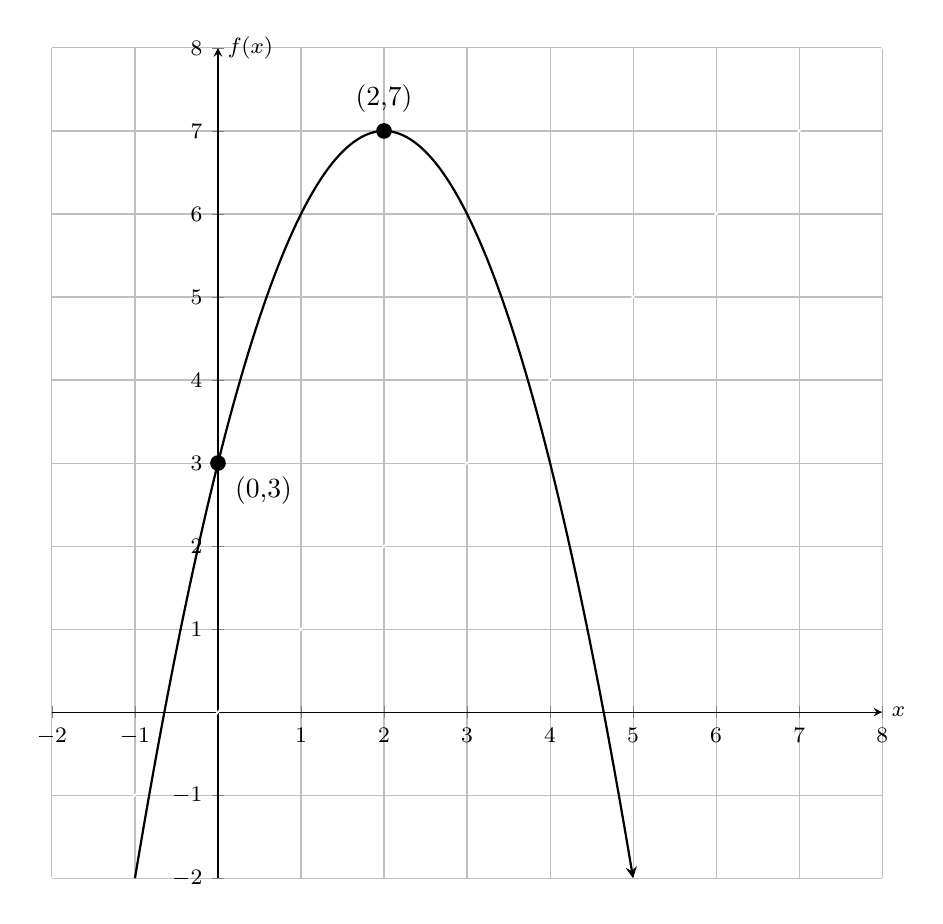
\begin{tikzpicture}
        \begin{axis}[
            my axis style,
            width=\textwidth,
            height=\textwidth,
            ylabel=$f(x)$,
            grid
        ]
        
        \addplot[
            domain=-2:8,
            thick,
            white,
            -
        ]
        {x};

        \addplot[
            domain=-1:5,
            thick,
            black,
            ->
        ]
        {-(x-2)^2 + 7};

        \fill[
            black
        ];


        \node[label={90:{($2$,$7$)}},circle,fill,inner sep=2pt] at (axis cs:2,7) {};
        \node[label={330:{($0$,$3$)}},circle,fill,inner sep=2pt] at (axis cs:0,3) {};
     

        \end{axis}
        \end{tikzpicture}
    \end{center}
  \end{enumerate}
\end{qstn}

\newpage


\begin{qstn}
  (2 marks) We call a function \emph{idempotent} if $f(f(x)) = f(x)$. Is the function \\
  $f(x) = x$ \emph{idempotent}? Justify your answer.
\end{qstn}
\begin{solution}
  Yes it is,  $f(x) = x$ is the function that returns whatever is input, and hence
  \[
        f(f(x)) = f(x)
  .\] 
\end{solution}

\begin{qstn}
  (7 marks) Factor the following quadratic functions,
  \begin{enumerate}[label=(\alph*)]
    \item $f\left( x \right) = -x ^2 +9x -20$.
      \begin{solution}
        \begin{align*}
          f(x) &= -\left( x^2 - 9x + 20 \right) \\
               &= -(x-4)(x-5)
        .\end{align*}
      \end{solution}

    \item $f(x) = 4x^2 - 1$.
      \begin{solution}
        \begin{align*}
          f(x) &= \left(\sqrt{4}x + \sqrt{\left|-1\right|}   \right) \left( \sqrt{4} x - \sqrt{\left|-1\right|}  \right)\\
               &= (2x + 1)(2x - 1)
        .\end{align*}
      \end{solution}

    \item $f\left( x \right) = 2x^2 - 4x - 16$.\\
      \textbf{Hint:} This \emph{can} be factored simply.
      \begin{solution}
        \begin{align*}
          f(x) &= 2\left( x^2 - 2x - 8 \right) \\
               &= 2(x - 4)(x + 2)
        .\end{align*}
      \end{solution}
  \end{enumerate}
\end{qstn}

\newpage

\begin{qstn}
  (6 marks) Let $g(x) = 5x^2 + 14x - 3$,
  \begin{enumerate}[label=(\alph*)]
    \item How many solutions will $g(x)$ have? (\textbf{Note: }$14^2 = 196$)
      \begin{solution}
        We turn to the discriminant formula to help answer this inquiry,
        \begin{align*}
          d &= b^2 - 4ac\\
            &= (14)^2 - 4(5)(-3)\\
            &= 196 + 60\\
            &= 256
        .\end{align*}
        Hence since $d > 0$, $g(x)$ will have two \emph{distinct} solutions.
      \end{solution}

    \item Factor $g(x)$.
      \begin{solution}
        \begin{step}[1]
          Find $p,q$ such that,
          \begin{align*}
            p + q &= 14\\
            p \cdot q &= -15
          .\end{align*}
          After some thinking you should arrive at $p = 15$,  $q = -1$. (Again how you labelled them was up to you).
        \end{step}

        \begin{step}[2]
          Compute $t$ and $k$,
          \begin{itemize}
            \item $t = \gcd \left(\left|a\right|, \left|p\right|\right) = \gcd \left(5,15\right) = 5$.
            \item $k = \gcd \left( \left|q\right|, \left|c\right| \right) = \gcd \left( \left|-1\right|, \left|-3\right| \right) = \gcd \left( 1,3 \right) = 1 $.
          \end{itemize}
        \end{step}

        \begin{step}[3]
          Since $a \cdot  q = 5 \cdot  (-1) = -5$, we conclude that $a \cdot  q < 0$ and hence,
          \[
              g(x) = \left( tx - k \right) \left( \frac{a}{t}x + \frac{p}{t} \right) = (5x - 1)(x + 3)
          .\] 
        \end{step}
        \qed
      \end{solution}

  \end{enumerate}
\end{qstn}

\begin{qstn}
  (6 marks) Let $T(x) = -\frac{1}{2}(2x - 22)(x + 1)$. Convert $T(x)$ into vertex form.
  \begin{solution}
    \begin{step}[1]
      Set both factors equal to null and solve,
      \begin{align*}
        2x - 22 &= 0\\
        2x &= 22\\
        x_1 &= 11\\
        \\
        x + 1 &= 0\\
        x_2 &= -1\\
      \end{align*}
    \end{step}

    \begin{step}[2]
      Calculate $h$,
      \[
          h = \frac{x_1 + x_2}{2} = \frac{11 + (-1)}{2} = \frac{10}{2} = 5
      .\] 
    \end{step}

    \begin{step}[3]
      Calculate $k$,
      \begin{align*}
        k &= T(h)\\
          &= T(5)\\
          &= -\frac{1}{2}(2(5) - 22)(5 + 1)\\
          &= -\frac{1}{2}(10 - 22)(6)\\
          &= -\frac{1}{2}(-12)(6)\\
          &= (6)(6)\\
          &= 36
      .\end{align*}

    \end{step}

    \begin{step}[4]
      Calculate $a$,
      \[
          a = b \cdot m \cdot  n = \left( -\frac{1}{2} \right) (2)(1) = -1
      .\] 
    \end{step}

    \begin{step}[5]
      Finalize,
      \[
            T(x) = a(x-h)^2 + k = -(x - 5)^2 + 36
      .\] 
    \end{step}

  \end{solution}
\end{qstn}

\newpage

\begin{qstn}
  (6 marks) A function is \emph{nilpotent} if there exists some number $t$ such that \\
  $f(f(t)) = 0$. Let  $T(x) = x^2 - 1$.
  \begin{enumerate}[label=(\alph*)]
    \item Determine $T(T(1))$.
      \begin{solution}
        \begin{step}[1]
          Compute $T(1)$,
           \[
              T(1) = (1)^2 - 1 = 1 - 1 = 0
          .\] 
        \end{step}

        \begin{step}[2]
          Compute $T(T(1))$,
           \[
              T(T(1)) = T(0) = 0^2 - 1 = -1
          .\] 
        \end{step}
      \end{solution}

    \item Determine $T(T(0))$.
      \begin{solution}
        \begin{step}[1]
          We need to compute $T(0)$, however we did that in part (a) and got  $T(0) = -1$.
        \end{step}

        \begin{step}[2]
          Compute $T(T(0))$,
           \[
                T(T(0)) = T(-1) = (-1)^2 - 1 = 1 - 1 = 0
          .\] 
        \end{step}
      \end{solution}

    \item Is $T(x)$ \emph{nilpotent}? Justify your answer.
      \begin{solution}
        Yes it is because $T(T(0)) = 0$. If you want to be thorough, then let $t = 0$, this would imply that
         \[
              T(T(t)) = T(T(0)) = 0 = t
        .\] \qed
      \end{solution}

  \end{enumerate}
\end{qstn}

\begin{qstn}
  (6 marks) Let $f(x) = x - 1$ and $g(x) = x + 1$. We call $f$ and $g$ \emph{mutual inverses} of each other if \textbf{both} of the following conditions
  hold,
  \begin{itemize}
    \item For every number $b$,  $f(g(b)) = b$.
    \item For every number $a$,  $g(f(a)) = a$.
  \end{itemize}

  \begin{enumerate}[label=(\alph*)]
    \item Determine $f(g(1))$.
      \begin{solution}
        \begin{step}[1]
          Compute $g(1)$,
           \[
                g(1) = 1 + 1 = 2
          .\] 
        \end{step}

        \begin{step}[2]
          Compute $f(g(1))$,
           \[
              f(g(1)) = f(2) = 2 - 1 = 1
          .\] 
        \end{step}
      \end{solution}
      \newpage

    \item Determine $g(f(2))$.
      \begin{solution}
        \begin{step}[1]
          Compute $f(2)$,
           \[
             f(2) = 2 - 1 = 1
          .\] 
        \end{step}

        \begin{step}[2]
          Compute $g(f(2))$,
           \[
              g(f(2)) = g(1) = 1 + 1 = 2
          .\] 
        \end{step}
      \end{solution}

    \item Based on your answers from part (a) and (b), do you think $f$ and $g$ are inverses of each other?
      \begin{solution}
        I would say so because they are satisfying the conditions of mutual inverses so far. (BTW, you can give a formal proof
        that they are indeed mutual inverses of each other, ill leave that as a challenge for however wants to try it)
      \end{solution}

  \end{enumerate}
\end{qstn}

\begin{qstn}
  (6 marks) Let $S = \{x \in \R \mid 8x^2 + 2x - 3 = 0\}$. Write down the elements of $S$.\\
  \textbf{Hint: }Try factoring first.
  \begin{solution}
    Lets follow the hint by factoring the quadratic given in the set.
    \begin{step}[1]
      Since $a \neq 1$, lets try factoring $f(x)$ by the non simple technique. Thus lets find the integers
      $p,q$ such that,
      \begin{align*}
        p + q &= 2\\
        p \cdot q &= -24
      .\end{align*}
      After thinking long enough you should arrive at $p = 6$ and $q = -4$ (How you label them is up to you).
    \end{step}

      \begin{step}[2]
        Compute $k$ and $t$,
        \begin{itemize}
            \item $t = \gcd \left(\left|a\right|, \left|p\right|\right) = \gcd \left(8,6\right) = 2$.
            \item $k = \gcd \left( \left|q\right|, \left|c\right| \right) = \gcd \left( \left|-4\right|, \left|-3\right| \right) = \gcd \left( 4,3 \right) = 1 $.
        \end{itemize}
      \end{step}

      \begin{step}[3]
       Since $a \cdot  q = 8 \cdot (-4) = -32$, we conclude that $a \cdot q < 0$ and hence,
       \[
            8x^2 + 2x - 3 = (tx - k)\left( \frac{a}{t}x + \frac{p}{t} \right) = (2x - 1)(4x + 3)
       .\] 
      \end{step}
      \begin{step}[4]
        At this point we have reduced the problem to determining the elements of ,
        \[
              S = \{x \in \R \mid (2x - 1)(4x + 3) = 0\}
        .\] 
        \newpage
      The question remains, when is $(2x - 1)(4x + 3) = 0$? This requires a subtle observation. When is the product of two numbers zero? In other words, when is $a \cdot b
      = 0$? If you think long enough, you'll conclude that this only happens when $a = 0$ or $b = 0$ (or both). Therefore we are
      left with the following two questions,
      \begin{itemize}
        \item For which $x$ is $2x - 1 = 0$?
        \item For which $x$ is $4x + 3 = 0$?
      \end{itemize}
      We proceed by answering our inquires,
      \begin{align*}
            2x - 1  &= 0\\
            2x &= 1\\
            x &= \frac{1}{2}\\
            \\
            4x + 3  &= 0\\
            4x &= -3\\
            x &= -\frac{3}{4}
      \end{align*}
      Hence the elements of $S$ are,
      \[
          S = \left\{ \frac{1}{2}, -\frac{3}{4} \right\} 
      .\] 
      \end{step}
  \end{solution}


\end{qstn}


\end{document}






























